\section{Date: 2026-09-29}
\noindent \textbf{Series ID: W269RE1A156NBEA} 

\noindent This series is titled Shares of gross domestic income: Compensation of employees, paid: Wage and salary accruals: Disbursements (DISCONTINUED) and has a frequency of Annual. The units are Percent and the seasonal adjustment is Not Seasonally Adjusted.The observation start date is 1929-01-01 and the observation end date is 2011-01-01.The popularity of this series is 1. \\ 

\noindent \textbf{Series ID: LNU05000006} 

\noindent This series is titled Not in Labor Force, Black or African American and has a frequency of Monthly. The units are Thousands of Persons and the seasonal adjustment is Not Seasonally Adjusted.The observation start date is 1972-01-01 and the observation end date is 2026-08-01.The popularity of this series is 1. \\ 

\subsection{Raw Regression}
\noindent Regresses the two series against each other directly. A significant result here can come just as easily from both series sharing a long-run trend as from any real relationship.

\begin{center}
\begin{tabular}{lclc}
\toprule
\textbf{Dep. Variable:}               & value\_fred\_LNU05000006 & \textbf{  R-squared:         } &     0.886   \\
\textbf{Model:}                       &           OLS            & \textbf{  Adj. R-squared:    } &     0.883   \\
\textbf{Method:}                      &      Least Squares       & \textbf{  F-statistic:       } &     295.5   \\
\textbf{Date:}                        &     Tue, 29 Sep 2026     & \textbf{  Prob (F-statistic):} &  1.63e-19   \\
\textbf{Time:}                        &         17:07:32         & \textbf{  Log-Likelihood:    } &   -300.21   \\
\textbf{No. Observations:}            &              40          & \textbf{  AIC:               } &     604.4   \\
\textbf{Df Residuals:}                &              38          & \textbf{  BIC:               } &     607.8   \\
\textbf{Df Model:}                    &               1          & \textbf{                     } &             \\
\textbf{Covariance Type:}             &        nonrobust         & \textbf{                     } &             \\
\bottomrule
\end{tabular}
\begin{tabular}{lcccccc}
                                      & \textbf{coef} & \textbf{std err} & \textbf{t} & \textbf{P$> |$t$|$} & \textbf{[0.025} & \textbf{0.975]}  \\
\midrule
\textbf{const}                        &    3.833e+04  &     1754.440     &    21.850  &         0.000        &     3.48e+04    &     4.19e+04     \\
\textbf{value\_fred\_W269RE1A156NBEA} &    -632.0219  &       36.768     &   -17.190  &         0.000        &     -706.454    &     -557.590     \\
\bottomrule
\end{tabular}
\begin{tabular}{lclc}
\textbf{Omnibus:}       &  2.321 & \textbf{  Durbin-Watson:     } &    0.414  \\
\textbf{Prob(Omnibus):} &  0.313 & \textbf{  Jarque-Bera (JB):  } &    1.433  \\
\textbf{Skew:}          &  0.178 & \textbf{  Prob(JB):          } &    0.488  \\
\textbf{Kurtosis:}      &  2.143 & \textbf{  Cond. No.          } & 1.17e+03  \\
\bottomrule
\end{tabular}
%\caption{OLS Regression Results}
\end{center}

Notes: \newline
 [1] Standard Errors assume that the covariance matrix of the errors is correctly specified. \newline
 [2] The condition number is large, 1.17e+03. This might indicate that there are \newline
 strong multicollinearity or other numerical problems.

\begin{figure}
\centering
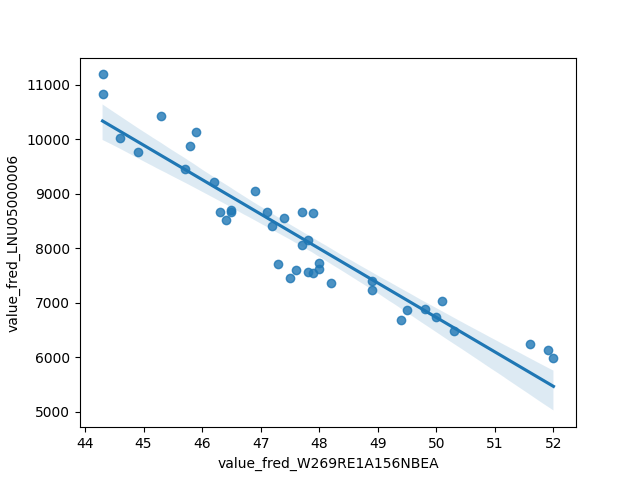
\includegraphics[scale = 0.9]{plots/plot_2026-09-29.png}
\caption{Raw Regression Plot for 2026-09-29}
\end{figure}
\newpage
\subsection{Detrended Regression}
\noindent Regresses the residuals of each series after removing its own linear time trend, so a shared trend can no longer drive the result on its own. A relationship that stays significant here is better evidence of a genuine link between the two series.

\begin{center}
\begin{tabular}{lclc}
\toprule
\textbf{Dep. Variable:}                          & value\_fred\_LNU05000006\_detrended & \textbf{  R-squared:         } &     0.229   \\
\textbf{Model:}                                  &                 OLS                 & \textbf{  Adj. R-squared:    } &     0.209   \\
\textbf{Method:}                                 &            Least Squares            & \textbf{  F-statistic:       } &     11.29   \\
\textbf{Date:}                                   &           Tue, 29 Sep 2026          & \textbf{  Prob (F-statistic):} &  0.00178    \\
\textbf{Time:}                                   &               17:07:32              & \textbf{  Log-Likelihood:    } &   -275.80   \\
\textbf{No. Observations:}                       &                    40               & \textbf{  AIC:               } &     555.6   \\
\textbf{Df Residuals:}                           &                    38               & \textbf{  BIC:               } &     559.0   \\
\textbf{Df Model:}                               &                     1               & \textbf{                     } &             \\
\textbf{Covariance Type:}                        &              nonrobust              & \textbf{                     } &             \\
\bottomrule
\end{tabular}
\begin{tabular}{lcccccc}
                                                 & \textbf{coef} & \textbf{std err} & \textbf{t} & \textbf{P$> |$t$|$} & \textbf{[0.025} & \textbf{0.975]}  \\
\midrule
\textbf{const}                                   &    4.404e-11  &       38.755     &  1.14e-12  &         1.000        &      -78.455    &       78.455     \\
\textbf{value\_fred\_W269RE1A156NBEA\_detrended} &    -174.7065  &       51.991     &    -3.360  &         0.002        &     -279.957    &      -69.456     \\
\bottomrule
\end{tabular}
\begin{tabular}{lclc}
\textbf{Omnibus:}       &  8.056 & \textbf{  Durbin-Watson:     } &    0.312  \\
\textbf{Prob(Omnibus):} &  0.018 & \textbf{  Jarque-Bera (JB):  } &    6.850  \\
\textbf{Skew:}          &  0.862 & \textbf{  Prob(JB):          } &   0.0325  \\
\textbf{Kurtosis:}      &  4.067 & \textbf{  Cond. No.          } &     1.34  \\
\bottomrule
\end{tabular}
%\caption{OLS Regression Results}
\end{center}

Notes: \newline
 [1] Standard Errors assume that the covariance matrix of the errors is correctly specified.

\begin{figure}
\centering
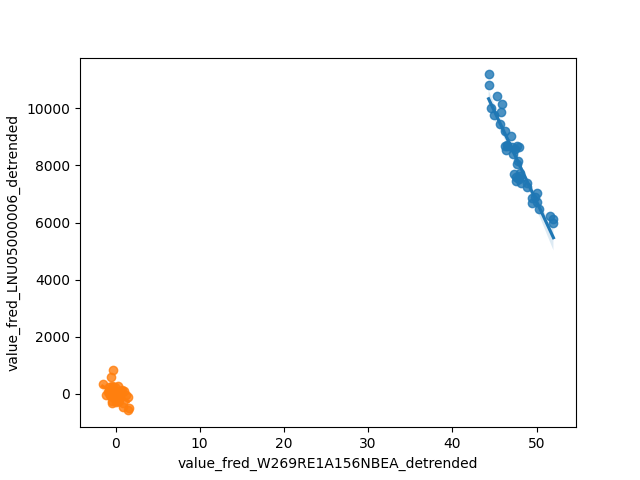
\includegraphics[scale = 0.9]{plots/plot_2026-09-29_detrended.png}
\caption{Detrended Regression Plot for 2026-09-29}
\end{figure}
\newpage
